\documentclass[9pt,a4paper,twoside]{tau}
\usepackage[english, italian]{babel}
\usepackage{tauenvs}

%----------------------------------------------------------
% TITLE
%----------------------------------------------------------

\title{Lighting and Shading: il modello del Ray Tracing}

%----------------------------------------------------------
% AUTHORS, AFFILIATIONS AND PROFESSOR
%----------------------------------------------------------

\author{Antonio Sirignano - Ciro Scognamiglio}

%----------------------------------------------------------

%\affil[a]{Affiliation of author one}
%\affil[b]{Affiliation of author two}
%\affil[c]{Affiliation of author three}

\professor{Calcolo Scientifico per l'Innovazione Tecnologica - prof. Luisa D'Amore}

%----------------------------------------------------------
% FOOTER INFORMATION
%----------------------------------------------------------

\institution{Università degli Studi di Napoli Federico II}
\ftitle{Lighting and Shading: il modello del Ray Tracing}
\date{a.a. 2023-2024}
\etal{Sirignano - Scognamiglio}
\course{Calcolo Scientifico per l'Innovazione Tecnologica}

%----------------------------------------------------------
% ABSTRACT
%----------------------------------------------------------

\begin{abstract}    
    In questo progetto viene fatta un'introduzione generale al lighting e allo shading, con una presentazione dei modelli di riflessione e di shading che possono essere applicati alla grafica computazionale.\\
    Nel seguito viene presentato in maniera più approfondita il modello del Ray Tracing, con le sue applicazioni, in particolare al mondo del video game e il 3D video editing.
\end{abstract}

%----------------------------------------------------------

\keywords{calcolo scientifico, lighting, shading, ray tracing.}

%----------------------------------------------------------

\begin{document}
		
	\maketitle
	\thispagestyle{firststyle}
	\tauabstract
	\tableofcontents

%----------------------------------------------------------

\section{Introduzione}

    \taustart{L}a Computer Graphic Technology è l'abilità d produrre un effetto visivo realistico in un oggetto tridimensionale in un device di output bidimensionale, come un computer o un foglio stampato.\\
    Tutto ciò si ha grazie ai \textit{metodi di rendering} nei quali è applicato lo \textit{shading} per raggiungere il più possibile una rappresentazione di un oggetto vicina alla realtà.\\ 
    Infatti lo shading computa quantità e colore della luce emessa da ogni punto della superficie.\\
    Tali risultati dipendono dalle seguenti entità:
    \begin{enumerate}
    	\item \textbf{La sorgente di luce}. Intensità, colore, forma, direzione e distanza della sorgente di luce devono essere prese in considerazione e inoltre possono essere sia puntiformi che di grandi dimensioni.
    	\item \textbf{La superficie dell'oggetto}. L'oggetto può essere lucido, liscio, ruvido, brillante o scuro. Può inoltre avere colori differenti quali opachi, trasparenti o traslucidi. 
    	\item \textbf{L'ambiente}. Oggetti visti in uno spazio vuoto, senza un background che rifletta la luce su di essi, risultano duri (una navicella spaziale nello spazio profondo). Un modello realistico di shading deve tenere in considerazione la luce riflessa dagli altri oggetti (pareti vicine).
    \end{enumerate}

\section{Le sorgenti di luce}
\taustart{U}n oggetto illuminato dalla luce è colpito da raggi luminosi proiettati sulla sua superficie da un emittente chiamato \textit{sorgente di luce}. La luce può descrivere diverse scene presentate di seguito.
\begin{enumerate}
    	\item \textbf{Luce ambientale}. Questa luce è una sorgente di luce non direzione la cui luce è emessa da ogni direzione. La sua intensità è indipendente da tutte le sue caratteristiche, come posizione e orientamento.
    		\begin{figure}[H]
        		\centering
       			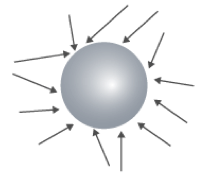
\includegraphics[width=0.6\columnwidth]{Figures/01.png}
       	 		\caption{Luce ambientale}
        		\label{fig:figure}
			\end{figure}
		
    	\item \textbf{Luce puntiforme}. \'E una sorgente di luce che non emette la stessa quantità di luce proveniente da tutte le direzioni, infatti un oggetto quanto è più vicino ad essa tanto è più luminoso. L'intensità della sorgente è quindi dipendente dalla distanza e dalla angolazione. \'E caratterizzata da colore, intensità, posizione e funzione di decadimento.
    		\begin{figure}[H]
        		\centering
        		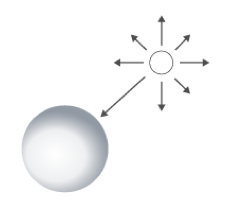
\includegraphics[width=0.6\columnwidth]{Figures/02.png}
        		\caption{Luce puntiforme}
       			\label{fig:figure}
			\end{figure}   
    	
    	\item \textbf{Luce direzionale}. Tale tipo è prodotta da una sorgente di luce da una distanza infinita dalla scena. Tutti i raggi di luce si espandano in una singola direzione e con la stessa intensità ovunque. \'E caratterizzata da colore, intensità e direzione.
    		\begin{figure}[H]
        		\centering
        		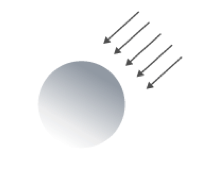
\includegraphics[width=0.6\columnwidth]{Figures/03.png}
        		\caption{Luce direzionale}
        		\label{fig:figure}
			\end{figure}
    	\item \textbf{Spotlight}. La luce si irradia in un cono con più luce al centro di esso. Questa luce è fissata all'asse primario di direzione con una restrizione su di essa. \'E caratterizzata come un punto di propagazione, un asse di direzione, un raggio intorno all'asse e la possibilità di una funzione di decadimento radiale. 
    		\begin{figure}[H]
		        \centering
		        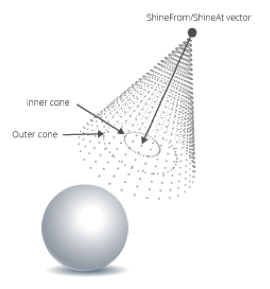
\includegraphics[width=0.6\columnwidth]{Figures/04.png}
		        \caption{Spotlight}
		        \label{fig:figure}
			\end{figure}
\end{enumerate}

\section{Modelli di riflessione}
\taustart{L'}obiettivo principale dello shading è la produzione di un risultato accettabile quando la superficie dell'oggetto è affetta dai raggi di luce. I modelli di riflessione sono presentati di seguito.
\begin{enumerate}
	\item \textbf{Riflessione diffusa}. Tale modello di riflessione diffonde la luce uniformemente in tutte le direzioni. In accordo con la legge di Lambert si ha che la diffusione del riflesso è proporzionale al coseno dell'angolo $\theta$ compreso tra la normale $N$ e la direzione della sorgente $L$. 
		\begin{figure}[H]
	        \centering
	        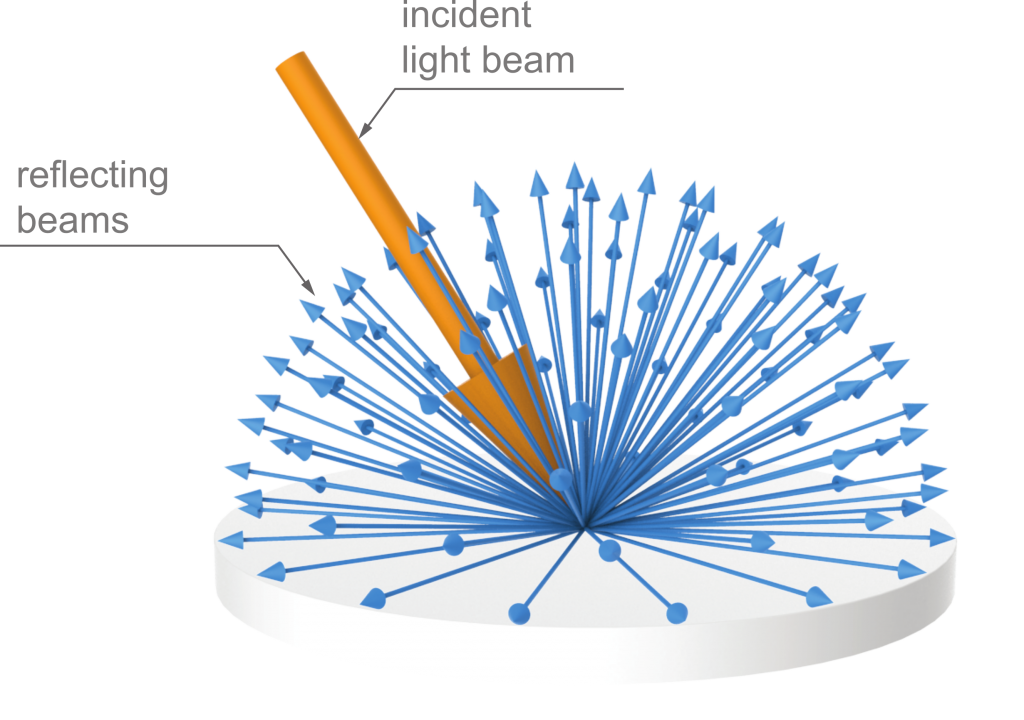
\includegraphics[width=0.6\columnwidth]{Figures/05.png}
	        \caption{Riflessione diffusa}
	        \label{fig:figure}
		\end{figure}
		Da qui
		\begin{equation*}
			\cos{\theta} = L \cdot N
		\end{equation*}
		E considerando il coefficiente di riflessione $k_d$, con $0\leq k_d \leq 1$, si ha
		\begin{equation*}
			R_d = k_d \cdot L \cdot N
		\end{equation*}
		Volendo considerare l'attenuazione della luce, si deve far riferimento alla distanze che essa percorre $d$. Quindi il termine di attenuazione quadratico è
		\begin{equation*}
			R_d = \frac{k_d}{A + BD + C(D \cdot D)}(L \cdot N)
		\end{equation*}
		E quindi
		\begin{equation*}
			I_d = \frac{k_d}{A + AD + A(D\cdot D)}(L \cdot N)
		\end{equation*}
	\item \textbf{Riflessione speculare}. Tale modello produce una riflessione luminosa sulla superficie dell'oggetto.
		\begin{figure}[H]
	        \centering
	        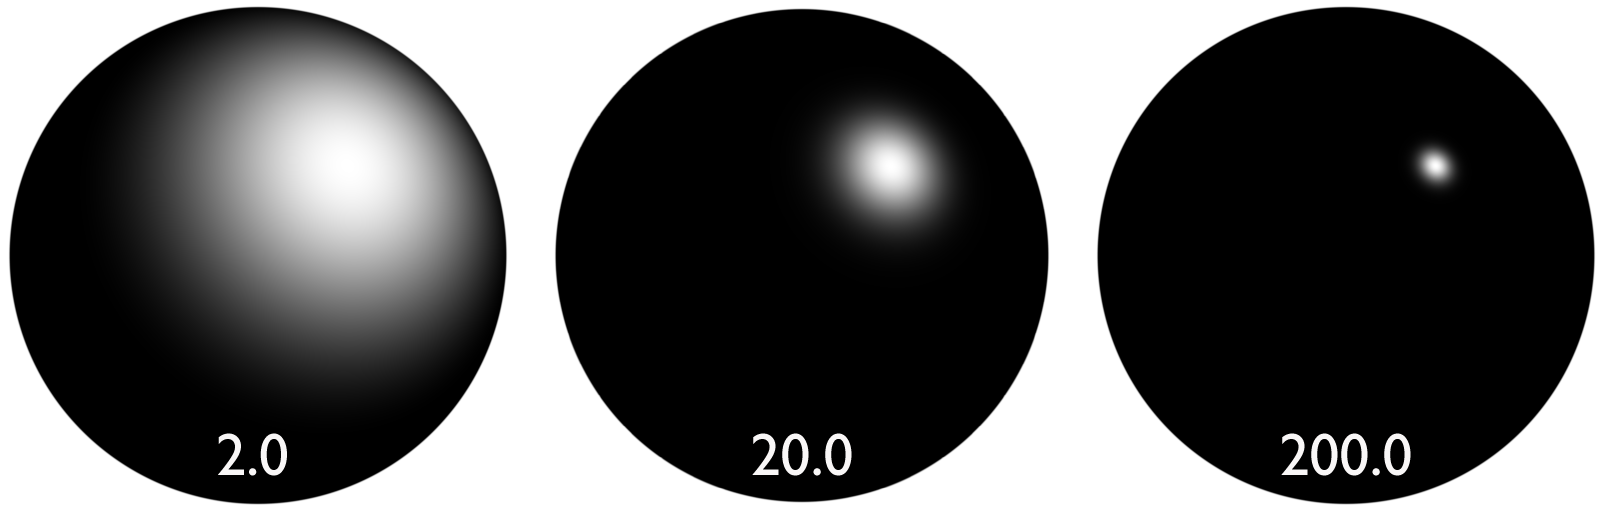
\includegraphics[width=0.6\columnwidth]{Figures/06.png}
	        \caption{Riflessione speculare}
	        \label{fig:figure}
		\end{figure} 
		L'angolo $\phi$ compreso tra la direzione della riflessione $r$ e la direzione $\nu$ dell'osservatore è affetto da una quantità di luce speculare. Il modello Phong stabilisce
		\begin{equation*}
			R_s = k_s \cos{^n}{\phi}
		\end{equation*}
		per coefficiente $k_s$, con $0 \leq k \leq 1$. L'esponente $n$ è il coefficiente di lucentezza. All'incrementare di $n$, la luce riflessa si concentra in una regione superficiale più piccola, centrata in $r$. Valori tra il 100 e il 500 corrispondono a superfici metalliche, valori più piccoli corrispondono a ad illuminazioni più ampie. Quindi
		\begin{equation*}
			R_s = k_s(r \cdot \nu )^n
		\end{equation*}
		Una distanza viene moltiplicata similmente alle riflessioni diffuse.\\
		La combinazione di tre tipi di riflessione danno
		\begin{equation*}
			I=\frac{1}{A + BD + C(D \cdot D)}(K_d(L \cdot N)L_d + k_s(r \cdot \nu)nL_s) + K_aL_a
		\end{equation*}
		La direzione della riflessione $r$ è semplice da $n$ e $I$, assumendo che $n$ sia un'unità di lunghezza, inoltre si vede che
		\begin{equation*}
			\frac{L+r}{2}=(L \cdot n)n \implies r = 2(L \cdot n)n - L
		\end{equation*}
\end{enumerate}

\section{Modelli di shading}
\taustart{I} modelli di shading sono utilizzati per ottenere il modello di illuminazione desiderato. Modelli di shading efficienti per la superficie definita da un poligono si possono descrivere come seguono.
\begin{enumerate}
	\item \textbf{Constant shading}. Questo modello è il più semplice modello di shading anche conosciuto come faceted shading o flat shading. Lo stesso colore è applicato su ogni intero poligono con un rendering veloce. L'equità della luce è usata una sola volta per poligono. Data una singola normale al piano, l'equazione della luce e le proprietà del materiale sono usate per generare un singolo colore. Il poligono avrà tale colore.
		
	\item \textbf{Gouraud shading}. Questo modello è anche chiamato intensity interpolation shading o color interpolation shading. I colori sono interpolati attraverso il poligono e vi è la necessità di identificare ogni vertice. Il processo di rendering è più lento rispetto al modello flat. L'equità della luce è applicata ad ogni vertice e anche ogni colore è determinato dalla quantità di luce con le proprietà del materiale. La Scan-line interpolation è usata per assegnare un colore ad ogni punto di proiezione del poligono come la media pesata dei colori di dati vertici.
	\item \textbf{Phong shading}. Tale modello è più realistico degli altri perché il suo algoritmo considera l'unione delle normali dei vertici ad ogni punto del poligono per avere una normale locale. Inoltre, il calcolo è applicato per avere un'illuminazione totale nel rendering.
\end{enumerate}
\begin{figure}[H]
    \centering
    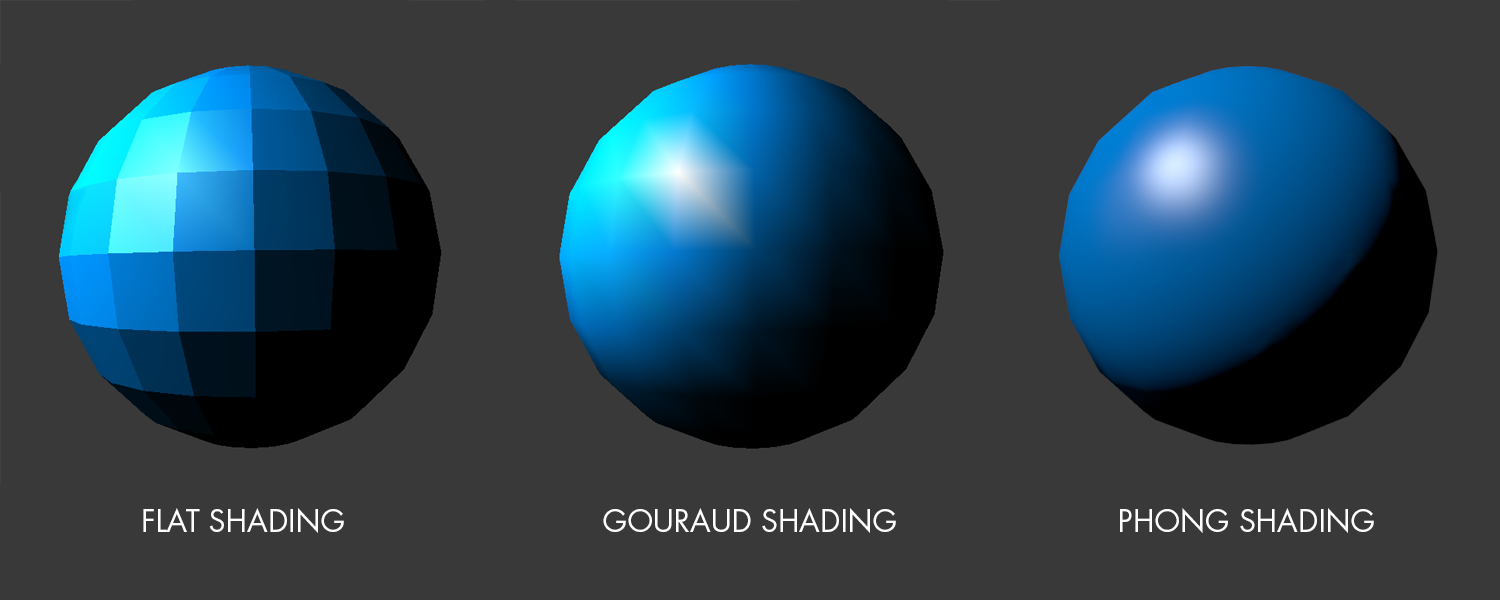
\includegraphics[width=0.7\columnwidth]{Figures/07.png}
    \caption{Flat, Gouraud e Phong shading}
    \label{fig:figure}
\end{figure}

%TODO parte di Ciro, cap 2-3		

\section{Il modello del Ray Tracing}
\taustart{L'}ambizione degli artisti, dei designers, degli ingegneri è sempre stata la simulazione dell'immagine di una scena, una storia, un prodotto, un palazzo prima che sia effettivamente realizzati e costruiti - architetti devono costruire modelli in scala, produttori di film e video-game devono utilizzare storyboards per provare e trasmettere le sensazioni di un film o un video-game. E gli inserzionisti vogliono creare interpretazioni perfette dei loro prodotti nella migliore luce possibile. Inoltre i designer di prodotti e macchinari vogliono trovare le debolezze di un progetto prima che esso venga effettivamente costruito - direttori di film vogliono vedere il risultato finale prima dell'arduo lavoro di post-produzione, i produttori vogliono mostrare a potenziali clienti il prodotto finale per stimolarne la domanda. Il test di tali idee è chiamato virtual prototyping nella manifattura e pre-visualization nell'industria cinematografica. Vi è quindi la necessità di disporre di queste immagini, o video, a basso costo e in poco tempo.\\

\section{L'equazione di rendering}
\taustart{N}ella computer graphics, l'equazione di rendering è un'equazione integrale nella quale la radianza di equilibrio che lascia un punto è la somma della radianza emessa più la radianza riflessa sotto un'approssimazione dell'ottica geometrica.
\begin{figure}[H]
    \centering
    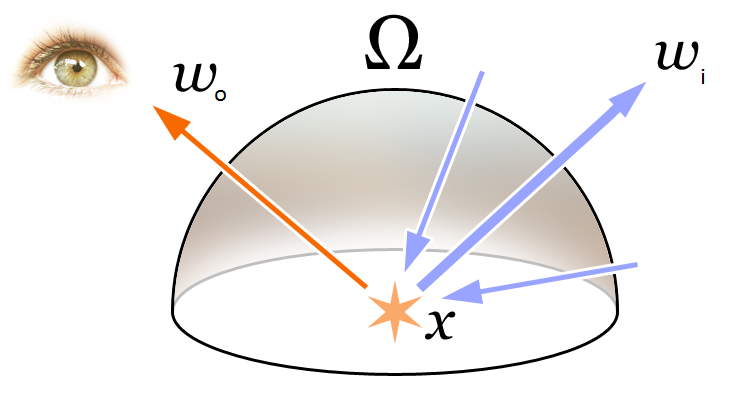
\includegraphics[width=0.7\columnwidth]{Figures/08.png}
    \caption{Equazione di rendering}
    \label{fig:figure}
\end{figure}
Esistono svariate tecniche di rendering nella computer graphics che cercano di risolvere tale equazione.
L'equazione di rendering descrive la quantità totale di luce emessa da un punto $x$ lungo una particolare direzione di osservazione, data una funzione per la luce in entrata e una funzione di distribuzione bidirezionale di riflettenza (BRDF), dove,
\begin{itemize}
	\item $x$ è una posizione nello spazio
	\item $w_o$ è la direzione della luce in uscita
	\item $\Omega$ è l'emisfero unitario centrato intorno $\{n\}$ contenente tutti i valori possibili di $w_i$
	\item $w_i$ è il fattore di indebolimento dell'irraggiamento verso l'esterno a causa dell'angolo di incidenza, poiché il flusso luminoso si diffonde su una superficie la cui area è più grande dell'area proiettata perpendicolare al raggio
\end{itemize}
Risolvere l'equazione di rendering per ogni scena è la prima sfida per ottenere un rendering realistico. \\
Uno degli approcci è basato sui metodi degli elementi finiti, che ha portato all'algoritmo di radiosità. Un altro approccio utilizzando il metodo Monte Carlo ha portato a diversi algoritmi inclusi Path Tracing, photon mapping, il Metropolis light transport e molti altri. Monte Carlo ray tracing richiede come input la descrizione di una scena altamente dettagliata e basata sulla fisica delle cose. L'algoritmo applica le leggi fisica per simulare la propagazione della luce attraverso la scena, piuttosto che approssimazioni ad hoc per i fenomeni visivi. Questo tipo di simulazione richiede modelli geometrici estremamente dettagliati. Inoltre, rendering fotorealistici richiedono che le proprietà fisiche del materiale superficiale siano modellate correttamente, in modo da descrivere come la luce si disperde quando la colpisce.

\section{Scanline rendering}
\taustart{L}o Scanline rendering è un algoritmo per la determinazione della superficie visibile che lavora riga per riga rispetto a poligono per poligono o pixel per pixel.
\begin{figure}[H]
    \centering
    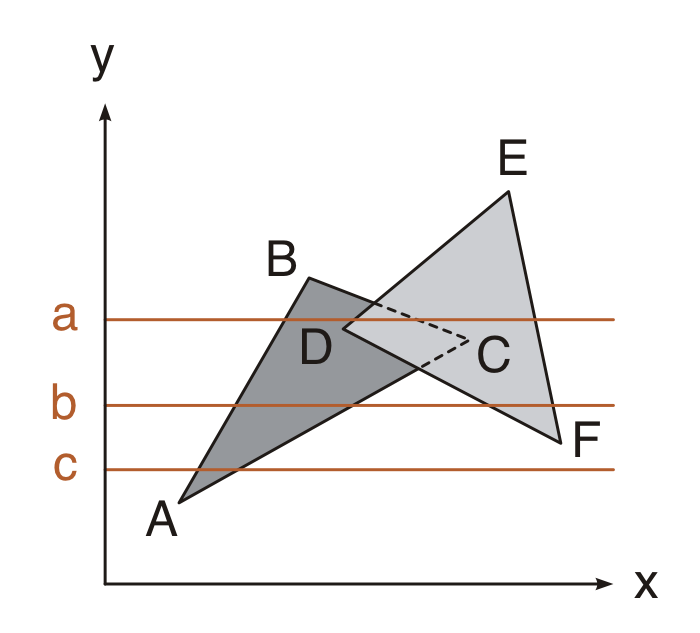
\includegraphics[width=0.7\columnwidth]{Figures/09.png}
    \caption{Algoritmo Scanline}
    \label{fig:figure}
\end{figure}
Tutti i poligoni da renderizzare sono ordinate dall'alto sulla asse delle ordinate in ordine di apparizione. Poi, per ogni riga o scanline dell'immagine è calcolato utilizzando l'intersezione di una scanline con i poligoni nella parte anteriore della lista ordinata, mentre quest'ultima viene aggiornata scartando i poligoni non più visibile man mano che la scanline attiva avanza verso il basso dell'immagine.\\
Il vantaggio principale di questo metodo è che l'ordine dei vertici lungo la normale del piano di scansione riduce il numero di comparazioni tra i bordi. Un ulteriore vantaggio rispetto allo z-buffering è che il processo dei pixel visibili è mantenuto al minimo assoluto. Attraverso l'ordinamento front-to-back utilizzato nei moderni sistemi z-buffer, si possono realizzare benefici simile. 

\subsection{Z-buffering}
Lo Z-buffering, anche noto come depth buffering, è la gestione delle coordinate di profondità delle immagini nella 3D graphics, fatta di solito a livello hardware. Quando si proietta un oggetto sullo schermo con un motore di 3D-rendering, la profondità (z-value) del pixel generato nell'immagine proiettata viene memorizzata in un buffer (z-buffer). Un z-value corrisponde alla misura della distanza perpendicolare da un pixel sul piano di proiezione alla sua corrispondete coordinata 3D su un poligono nello spazio. Lo Z-buffer ha la stessa struttura di un immagine, ovvero un 2D-array, con la sola differenza che memorizza uno z-value per ogni pixel dello schermo invece che dei pixel dei dati. Ha la stesse dimensioni di uno screen buffer, eccetto quando sono utilizzati Z-buffer multipli. \\
Quando vediamo un immagine contenente oggetti o superfici parzialmente o totalmente opachi, non è possibile vedere completamente questi oggetti sia che siano lontani dall'osservatore sia che siano dietro altri oggetti. L'identificazione e la rimozioni di tali oggetti è chiamato problema delle superfici nascoste (hidden surface problem). Per migliorare il tempo di rendering, le superfici nascoste vengono rimosse prima che l'immagina sia memorizzata nel z-buffer, in modo che quest'ultimo calcoli lo z-value del pixel corrispondente al primo oggetto che compare e lo compara con lo z-value del pixel nella stessa posizione nel z-buffer corrispondente all'oggetto che è più vicino all'osservatore per trovare la sovrapposizione.
\subsection{Algoritmo del pittore}
L'algoritmo del pittore è una delle soluzioni più semplici al problema della visibilità nella 3D computer graphics. Quando proietti una scena 3D in un piano 2D, è necessario decidere quale  tra i poligoni è visibile. 
\begin{figure}[H]
    \centering
    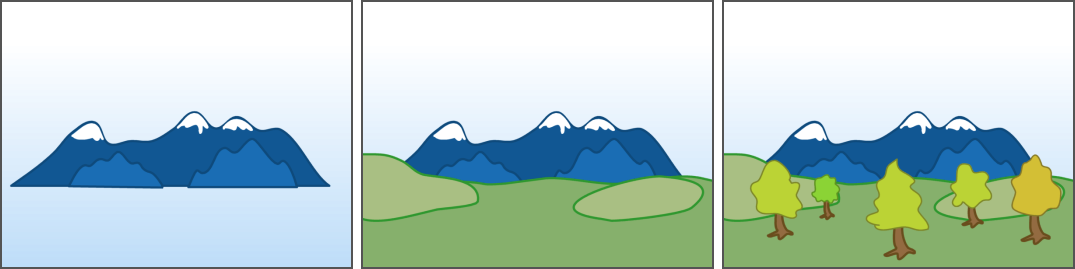
\includegraphics[width=0.7\columnwidth]{Figures/10.png}
    \caption{Algoritmo del pittore}
    \label{fig:figure}
\end{figure}
L'algoritmo del pittore ordina tutti i poligoni nella scena partendo dalla profondità e poi li disegna in questo ordine, dal più lontano al più vicino. Si disegna sulle parti non visibili, al costo di avere oggetti già disegnati al nascosti. L'ordine usato dall'algoritmo è chiamato depth order: se un oggetto oscura la parte di un altro, allora il primo oggetto disegnato dopo il secondo viene oscurato. 

\section{Ray Tracing}
Negli ultimi anni, la qualità delle immagini generate computazionalmente hanno raggiunto un livello di realismo tale che i rendering sono indistinti dalle fotografie.\\
Nella computer graphics, il ray tracing è una tecnica di rendering per generare un'immagine tracciando il percorso della luce come pixel in un piano e simulando gli effetti dati dall'intersezione di tale percorso con gli oggetti virtuali. La tecnica può produrre un grado di realismo visivo molto alto, anche più alto a volte dei tipici metodi di rendering scanline ma con un alto costo computazionale. \\
Avanzati effetti di shading possono rendere la visualizzazione più efficace. Il vantaggio, l'opportunità e l'obiettivo del ray tracing è quello di fornire ulteriori segnali visivi per una migliore visualizzazione degli oggetti 3D.\\
Ci sono almeno quattro diversi raggi coinvolti nel ray tracing:
\begin{itemize}
	\item \textbf{Raggi oculari} che hanno origine dagli occhi.
	\item \textbf{Raggi d'ombra}: dal punto di superficie alla sorgente di luce.
	\item \textbf{Raggi di riflessione}: dal punto di superficie in direzione dello specchio.
	\item \textbf{Raggi di trasmissione}: dal punto di superficie nella direzione di rifrazione.
\end{itemize}
L'algoritmo di ray tracing calcola il raggio dell'occhio dell'osservatore attraverso ogni pixel, calcola il punto di intersezione più vicina con una superficie di scena, quindi ombreggia quel punto calcolando i raggi d'ombra e genera i raggi riflessi e rifratti.
\begin{figure}[H]
    \centering
    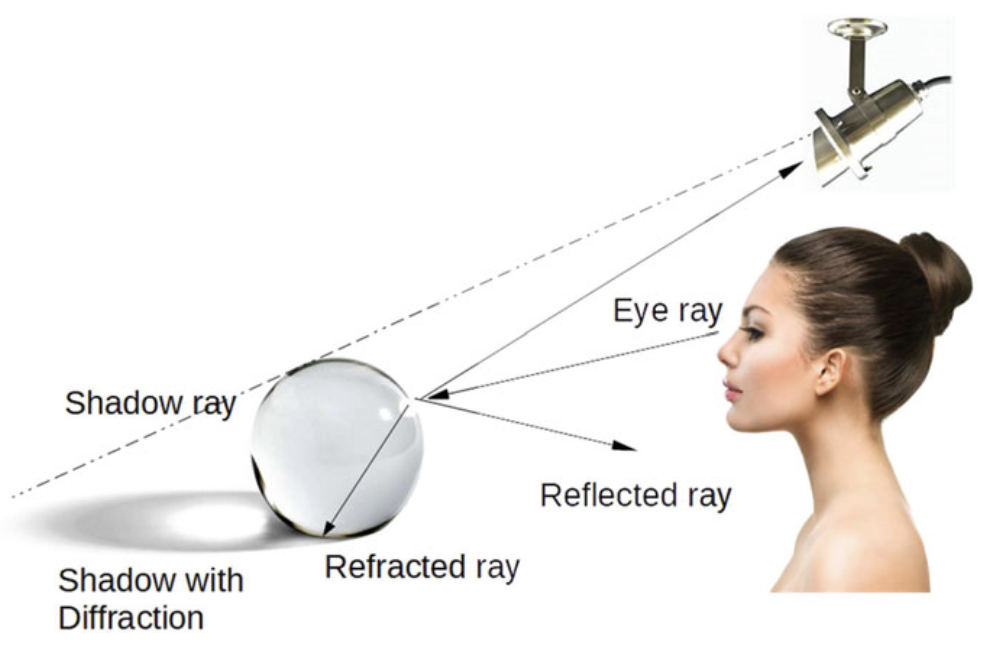
\includegraphics[width=0.7\columnwidth]{Figures/11.png}
    \caption{Raggi nel ray tracing}
    \label{fig:figure}
\end{figure}
Il ray tracing ricorsivo simula la riflessione speculare e le ombre attraverso e fuori dalle superfici trasparenti. Può usare o impiegare l'illuminazione indiretta, a volte aree di sorgenti luminosa o altre influenze caustiche.\\
Crea riflessi accurati, rifrazioni, ombre e altre caratteristiche che possano far sembrare la scena reale.\\
Il ray tracing in grandi linee può essere diviso in tre generali categorie:
\begin{enumerate}
	\item Off-line
	\item Interactive
	\item Real-time
\end{enumerate}
Off-line è usato ampiamente dagli studi cinematografici, pubblicitari e di design. Ha la qualità maggiore.\\
Interactive ray tracing riduce il numeri di raggi in modo da avere comunque una buona immagine e allo stesso tempo di offrire all'utente la possibilità di manipolare il modello.\\
Real-time ray tracing può essere realizzato, con alcune restrizioni, dall'assistenza di piccoli supercomputer.
\begin{figure}[H]
    \centering
    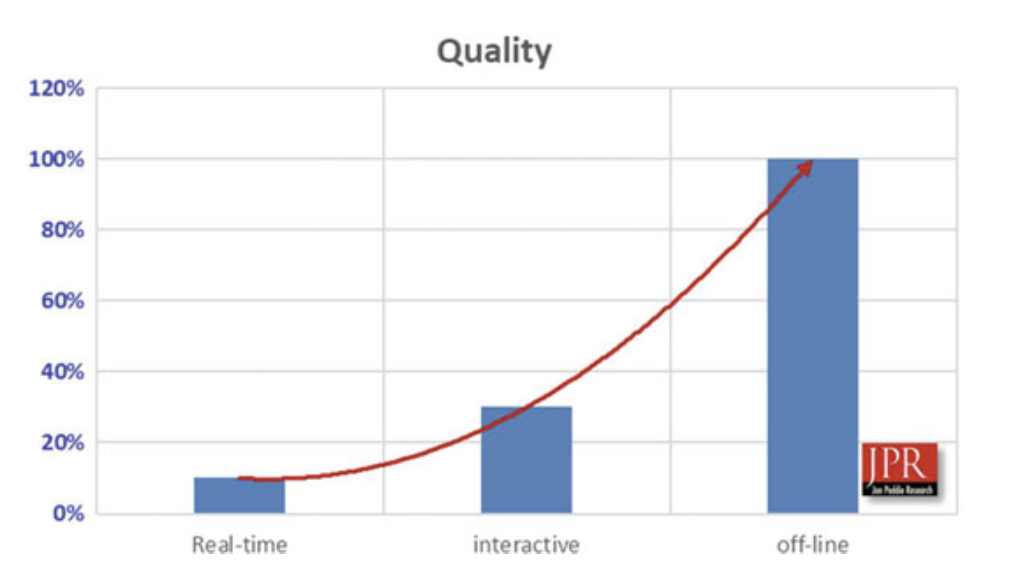
\includegraphics[width=0.7\columnwidth]{Figures/12.png}
    \caption{Performance e qualità nei vari modi di ray tracing}
    \label{fig:figure}
\end{figure}
Uno dei trucchi del ray tracing è quello di tracciare solo determinati elementi o oggetti all'interno di un'immagine ma, se fatto in modo giusto, si ha un immagine fisicamente corretta.  
\begin{figure}[H]
    \centering
    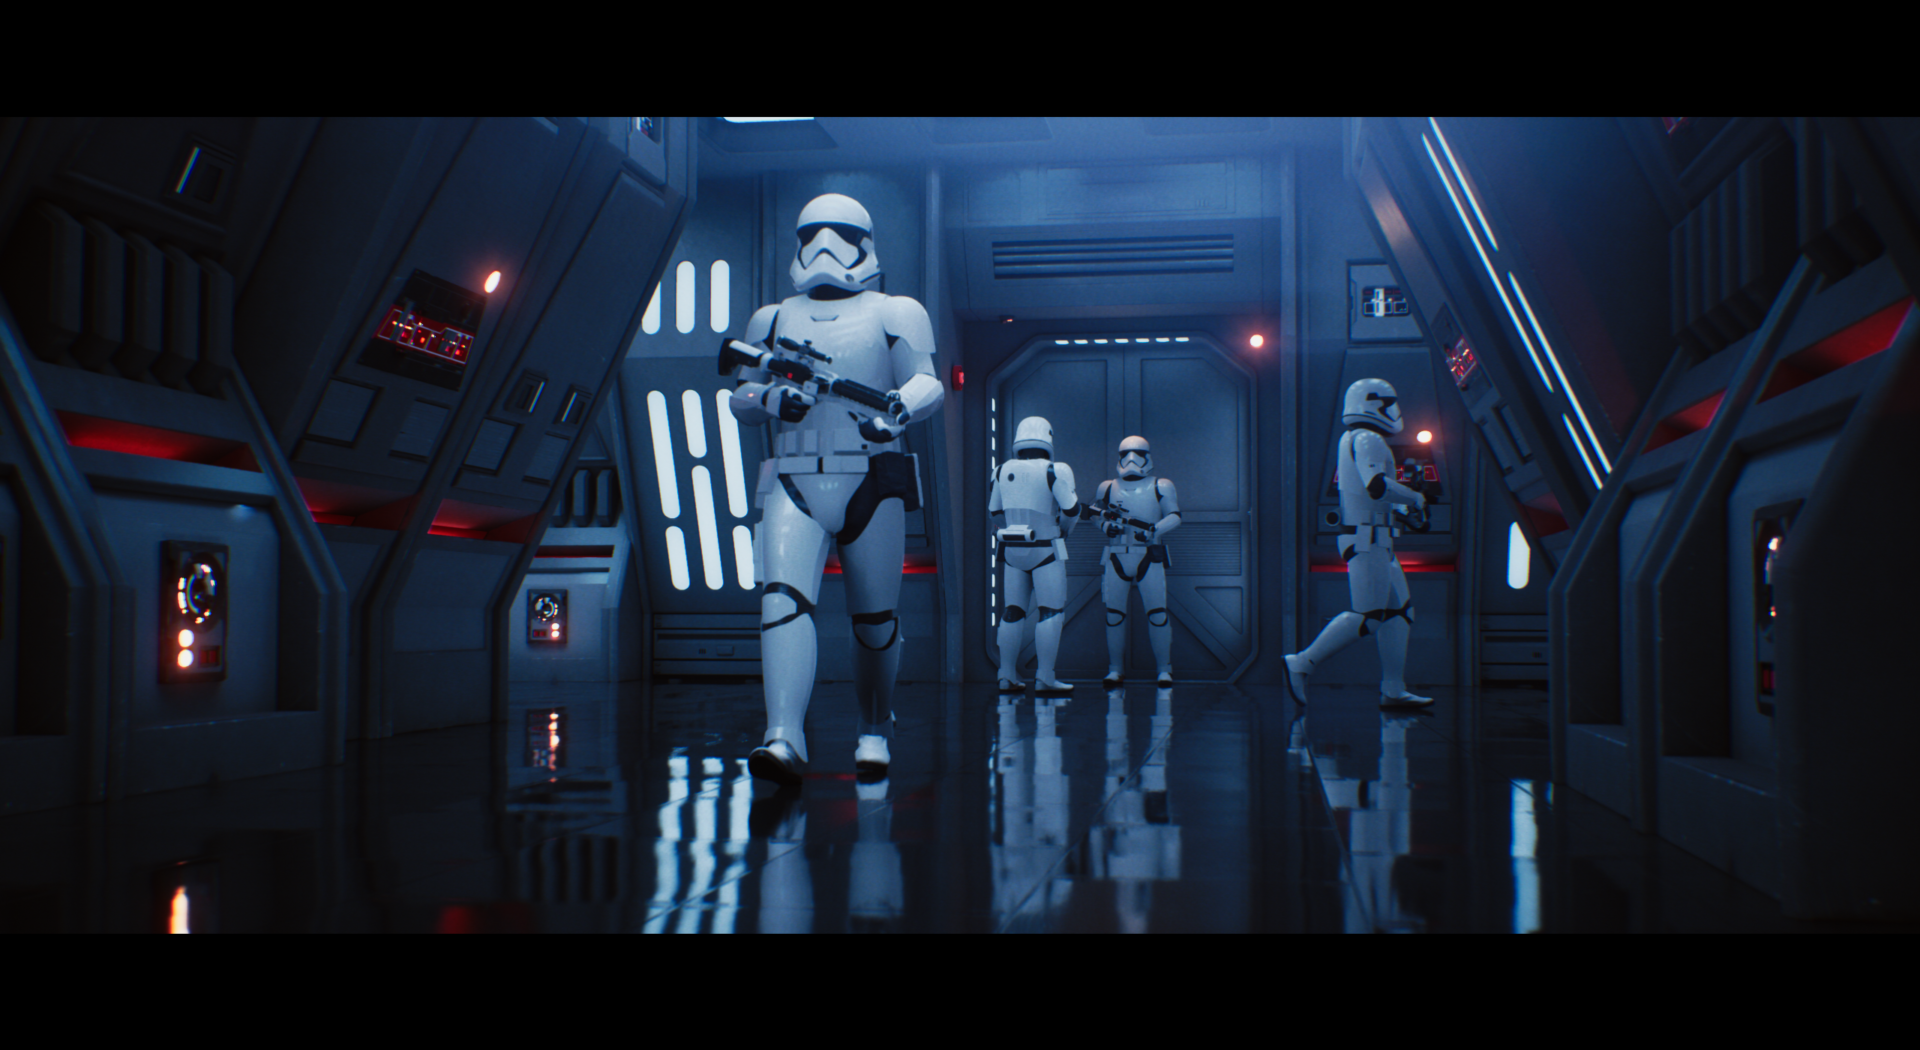
\includegraphics[width=0.7\columnwidth]{Figures/13.png}
    \caption{Stormtroopers (Star Wars) renderizzati con real-time ray tracing (Nvidia): il background non ha applicato il ray tracing, ne tanto meno lo necessita, ma il pavimento potrebbe dipendere dal materiale che il l'autore decida di utilizzare}
    \label{fig:figure}
\end{figure}
Il ray tracing è capace di simulare una vasta varietà di effetti ottici, ad esempio riflessione, rifrazione e fenomeni di dispersione, ma non è necessariamente il metodo più realistico: metodi che includono tecniche addizionali posso dare simulazioni più accurate. \\
Il ray tracing è imperfetto: immagini con un ray tracing basico sono molto pulite, quindi l'allineamento degli oggetti e il campionamento possono portare a pattern non intenzionali noti come pattern di moiré e aliasing. \\
Il ray tracing dà colore per ogni possibile punto dell'immagine. Tuttavia un pixel quadrato contiene un numero infinito di punti e quei punti potrebbero non avere tutti lo stesso colore. Il campionamento viene utilizzato appunto per scegliere il colore di tale pixel, ma come è ben noto, il campionamento implica aliasing.

\section{Path Tracing}
\taustart{I}l Path Tracing è un'estensione dell'algoritmo del ray tracing. Esso simula molti percorsi di luce per ogni pixel e ne valuta la media per calcolare il colore finale per ognuno di essi.\\
Ogni volta che un raggio colpisce una superficie, un nuovo raggio viene tracciato a partire dal punto di collisione in direzione casuale fino a quando raggiunge una massima profondità di percorso (maximum path depth) o finche un meccanismo "uccide" il raggio (simile ad una roulette russa). Di conseguenza, il Path Tracing produce effetti come mescolamento dei colori diffuso (diffuse color bleedind), riflessi lucisi (sfocati), ombre morbide, reali luci di area, vera profondità di campo.\\
Path Tracing usa il campionamento casuale (metodo Monte Carlo) per incrementare il calcolo dell'immagine finale: il processo di campionamento casuale consente di rendere alcuni fenomeni complessi che non vengono gestiti nel ray tracing regolare, ma generalmente ci vuole più tempo per produrre un'immagine tracciata di alta qualità. \\
Tale campionamento introduce del rumore nell'immagine renderizzata. Tale problema si risolve lasciando che l'algoritmo generi più campioni.

\subsection{Differenze tra Path Tracing e Ray Tracing}
Path Tracing si basa fisicamente sulla simulazione della luce che consente un rendering altamente realistico. \'E un algoritmo elegante che può simulare molti complessi modi di determinare il percorso e la dispersione della luce nelle scene virtuali. Il Path Tracing usa il tracciamento dei raggi per determinare la visibilità tra gli eventi di scattering. Ray Tracing è una operazione di base che può essere usata per molteplici cose. Quindi, il tracciamento dei raggi da solo non produce in maniera automatica immagini realistiche. Per questo si utilizzano algoritmi del trasporto della luce come il Path Tracing. Tuttavia, anche se elegante e molto potente, il Path Tracing è molto costoso e impiega parecchio tempo per produrre immagini stabili. A tal caso sono stati proposti dei filtri adattivi che riutilizzano più informazioni possibili su molti fotogrammi e pixel al fine di produrre immagini robuste e stabili.

\subsection{Rumore nel Ray Tracing}

\section{Applicazione}


%\section{Coding}
%
%    \textit{Tau class} includes the \textit{listings} package, which offers versatile and customizable features for typesetting code snippets in \LaTeX\ documents. Specifically for C, C++, \LaTeX\ and Matlab codes. 
%
%    For C and C++ codes, the \textit{listings} package recognizes the syntax of these programming languages and highlights keywords, comments, and string literals accordingly.
%
%    \lstinputlisting[caption=Example of C code., language=C]{example.c}
%
%    Similarly, for Matlab codes, the \textit{listings} package offers syntax highlighting and line numbering, to the MATLAB language syntax.
%    
%    \lstinputlisting[caption=Example of matlab code., language=Matlab]{example.m}
%
%\section{References}
%
%    The default formatting for references follows the IEEE style. This style is commonly used for technical documents, research papers, and scholarly articles in engineering fields \cite{einstein}.
%
%    At the end of the document, you will find an example of the default reference formatting \cite{dirac}.
%        
%\section{Appendix}
%
%    \subsection{Environments preview}
%
%        The following environments are defined in \textit{tauenvs} package.
%		
%		\subsubsection{Tau environment}
%
%                The following code defines the tauenv environment. A custom title can be added to this environment.
%
%			\begin{tauenv}[frametitle=Tauenv]
%                    Lorem ipsum dolor sit amet, consectetur adipiscing elit. Sed vestibulum justo quis massa aliquet, ut ultrices quam bibendum.
%			\end{tauenv}
%		
%\begin{lstlisting}[language=TeX, caption=Tauenv environment code.]
%\newmdenv[
%	backgroundcolor=taublue!22, 					
%	linecolor=taublue,									
%	linewidth=0.7pt,
%	frametitle=\vskip0pt\bfseries,
%	frametitlerule=false,
%	frametitlefont=\color{taublue}\bfseries\sffamily,
%	frametitlealignment=\raggedright,
%	innertopmargin=3pt,
%	innerbottommargin=6pt,
%	innerleftmargin=6pt,
%	innerrightmargin=6pt,
%	font=\selectfont,
%	fontcolor=taublue,									
%	frametitleaboveskip=8pt,
%	skipabove=10pt
%]{tauenv} \end{lstlisting}
%		
%		\subsubsection{Note}
%
%                This code defines the note environment.
%
%  			\begin{note}
%                    Lorem ipsum dolor sit amet, consectetur adipiscing elit. Sed vestibulum justo quis massa aliquet, ut ultrices quam bibendum.
%			\end{note}
%		
%\begin{lstlisting}[language=TeX, caption=Note environment code.]
%\newmdenv[
%	backgroundcolor=taublue!22, 						
%	linecolor=taublue,									
%	linewidth=0.7pt,
%	frametitle=\vskip0pt\bfseries\notelanguage,
%	frametitlerule=false,
%	frametitlefont=\color{taublue}\bfseries\sffamily,
%	frametitlealignment=\raggedright,
%	innertopmargin=3pt,
%	innerbottommargin=6pt,
%	innerleftmargin=6pt,
%	innerrightmargin=6pt,
%	font=\normalfont,
%	fontcolor=taublue,									
%	frametitleaboveskip=3pt,
%	skipabove=10pt
%]{note} \end{lstlisting}
%
%		\subsubsection{Info}
%
%                This code defines the info environment.
%
%    		\begin{info}
%                    Lorem ipsum dolor sit amet, consectetur adipiscing elit. Sed vestibulum justo quis massa aliquet, ut ultrices quam bibendum.
%			\end{info}
%		
%\begin{lstlisting}[language=TeX, caption=Info environment code.]
%\newmdenv[
%	backgroundcolor=taublue!22, 						
%	linecolor=taublue,									
%	linewidth=0.7pt,
%	frametitle=\vskip0pt\bfseries\infolanguage,
%	frametitlerule=false,
%	frametitlefont=\color{taublue}\bfseries\sffamily,
%	frametitlealignment=\raggedright,
%	innertopmargin=3pt,
%	innerbottommargin=6pt,
%	innerleftmargin=6pt,
%	innerrightmargin=6pt,
%	font=\normalfont,
%	fontcolor=taublue,									
%	frametitleaboveskip=3pt,
%	skipabove=10pt
%]{info} \end{lstlisting}
%
%    \subsection{Alternative title}
%
%         You can make the following modification to \textit{tau class} in the \textit{title preferences} section to change the position of the title. This will move the title to the left. 
%
%\begin{lstlisting}[language=TeX, caption=Alternative title.]
%\renewcommand{\@maketitle}{%
%        \vskip-18pt
%    {\RaggedRight\bfseries\color{taublue}\fontsize{18}{22}\sffamily\selectfont\@title\par}
%		\vskip8pt
%    {\RaggedRight\normalsize\sffamily\@author\par}
%        \vskip8pt
%    {\RaggedRight\fontsize{7pt}{8pt}\selectfont\@professor\par}
%        \vskip24pt
%}% 
%\end{lstlisting}
%
%    \subsection{Equation skip value}
%
%        Play with the value of \verb|\eqskip| until the preferred spacing is set for equations.
%
%\begin{lstlisting}[language=TeX, caption=Equation skip code.]
%\newlength{\eqskip}\setlength{\eqskip}{6.5pt}
%\expandafter\def\expandafter\normalsize\expandafter{%
%    \normalsize%
%    \setlength\abovedisplayskip{\eqskip}%
%    \setlength\belowdisplayskip{\eqskip}%
%    \setlength\abovedisplayshortskip{\eqskip-\baselineskip}%
%    \setlength\belowdisplayshortskip{\eqskip}%
%}
%\end{lstlisting}
					
%----------------------------------------------------------

\addcontentsline{toc}{section}{Riferimenti}
\nocite{*}
\printbibliography

%----------------------------------------------------------

\end{document}